\documentclass{article}

%%% Fill details here (in the second brackets)
\newcommand{\name}{Xin Qiu}     % Your name (First Last)
\newcommand{\wustlkey}{qiuxin}             % Your WUSTL Key
%%%



%%%%%%%%%%%%%%%%%%%%%% Formatting Stuff %%%%%%%%%%%%%%%%%%%%%%%%%%%
\usepackage{times}
\usepackage[T1]{fontenc}

\setlength{\parskip}{1em}\setlength{\parindent}{0pt}
\linespread{1.25}
\usepackage[margin=0.7in,top=1in]{geometry}\usepackage{fancyhdr}
\pagestyle{fancy}\lhead{\bf \name}\rhead{\bf \wustlkey}\cfoot{\thepage}
\newcommand{\info}{\clearpage \subsection*{Information}}
\newcommand{\solution}[1]{\clearpage \subsection*{Solution #1}}
\newcommand{\spart}[1]{\paragraph{(#1)}}
%%%%%%%%%%%%%%%%%%%%%%%%%%%%%%%%%%%%%%%%%%%%%%%%%%%%%%%%%%%%%%%%%%%


%%% Add any more packages if you want to
\usepackage{amsmath,graphicx}


\begin{document}
%%%%% Main Body goes here

% Begin solution to every problem like this.
\solution{1}
\spart{a}The probability that all of them are inliers is:
$$
P_r = \frac{C_{N-J}^{K}}{C_{N}^{K}}
$$
and $C_{N-J}^{K}=\frac{(N-J)!}{K!(N-J-K)!}$, $C_{N}^{K}=\frac{N!}{(N-K)!K!}$

\spart{b} Assume that the minimum number of times we should sample is $T$, then we have:
\begin{eqnarray*}
1 - (1 - \frac{C_{N-J}^{K}}{C_{N}^{K}})^{T} &\ge& P \\
                          1 - P & \ge & (1 - \frac{C_{N-J}^{K}}{C_{N}^{K}})^{T}\\
                          \log {(1-P)} &\ge& T\cdot \log {(1 - \frac{C_{N-J}^{K}}{C_{N}^{K}})}\\
                          T &\ge&\frac{\log {(1-P)}}{\log {(1 - \frac{C_{N-J}^{K}}{C_{N}^{K}})}}
\end{eqnarray*}
so, the minimum number of times is $\frac{\log {(1-P)}}{\log {(1 - \frac{C_{N-J}^{K}}{C_{N}^{K}})}}$.

\spart{c} The probability that all K samples are inliers and come from the same plane is:
$$
P_r = \frac{C_{I_1}^{K} + C_{I_2}^{K}}{C_N^K}
$$
and $C_{I_1}^{K} = \frac{{I_1}!}{K!(I_1 - K)!}$, $C_{I_2}^{K} = \frac{{I_2}!}{K!(I_2 - K)!}$, $C_{N}^{K}=\frac{N!}{(N-K)!K!}$.

\solution{2} 

\spart{a} Figure \ref{fig:prob2a} shows the result of implementation of the iterative fitting idea.

\begin{figure*}[!h]
  \centering
  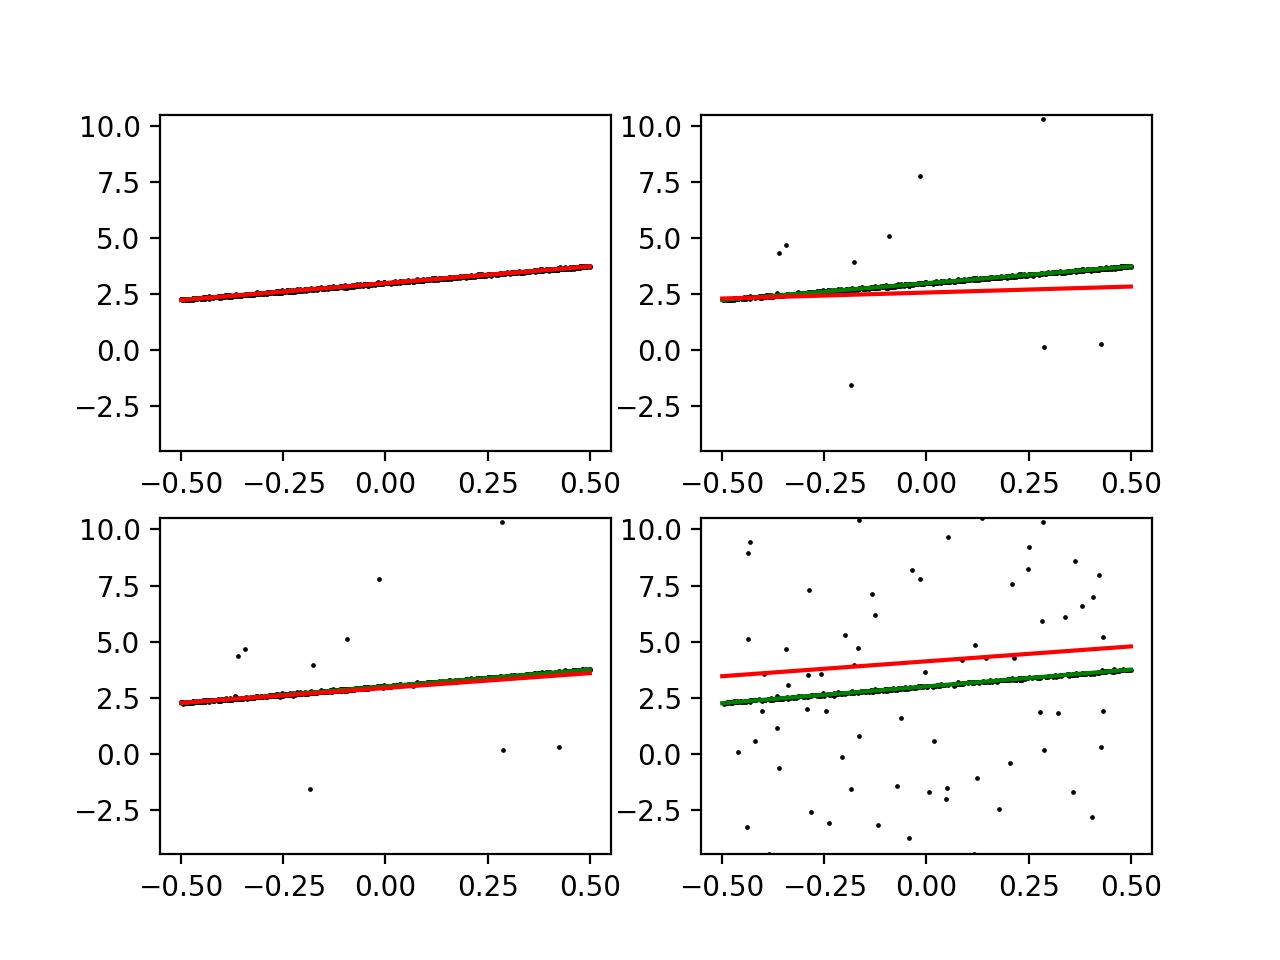
\includegraphics[height=20em]{code/outputs/prob2a.png}
  \caption{Implementation of the iterative fitting idea}
  \label{fig:prob2a}
\end{figure*}

\begin{enumerate}
\item For the top left image with single least-squares fit works well when there is no outliers and also with low variance noise.
\item Compare the top right image to the bottom left image, they have the same outliers, but the iterative estimation works better.
\item When we compare the bottom left image to the bottom right image, we will see that with larger number of outliers, the iterative estimation will converge to poorer minimum and then it would in some cases increase its error to be larger than $\epsilon$.
\end{enumerate}

\spart{b} Figure \ref{fig:prob2b} shows the result of implementation of RANSAC.
\begin{figure*}[!h]
  \centering
  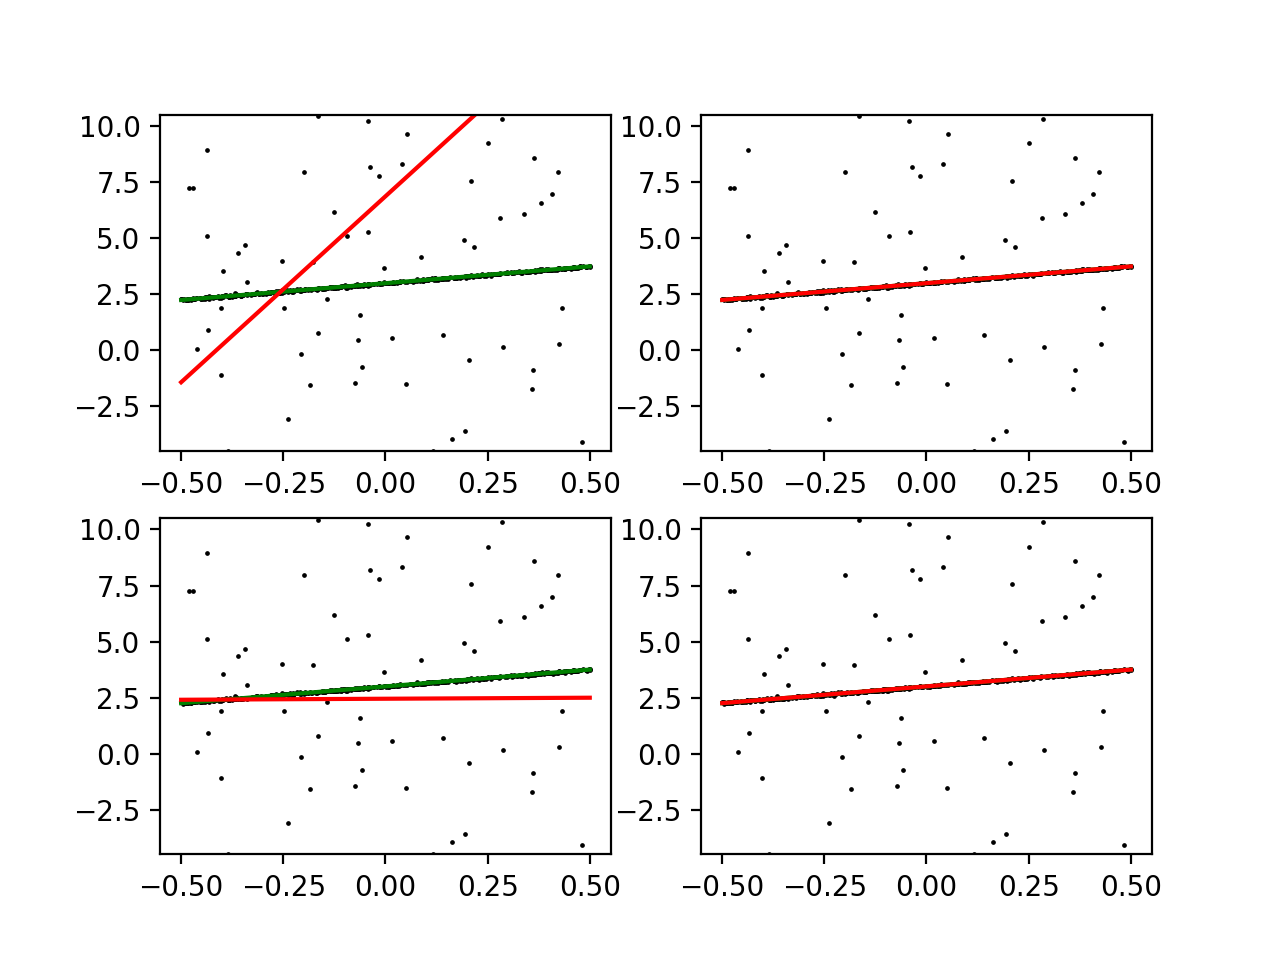
\includegraphics[height=20em]{code/outputs/prob2b.png}
  \caption{Implementation of RANSAC}
  \label{fig:prob2b}
\end{figure*}

As we can see from the above four images, with running the codes for multiple times, it shows that the top right image and the bottom right images works better than the other two images. The top right image and the bottom right image are both with K = 5. I think the reason is that K = 5 is sufficient because we are drawing 2D lines and the larger number of K, the lower probability of them are all inliers.

\solution{3}
\spart{a}Since we know the intrinsic projection matrix, and with $f = f_1$ for camera 1 and $f = f_2$ for camera two, so the relationship between the projection co-ordinates of the same point in two cameras can express as follows:
\begin{equation}
 \left[
      \begin{array}{c}
      x_2 \\ y_2 \\ 1
      \end{array}
 \right]
 =
 \left[
     \begin{array}{ccc}
     f_2 & 0 & \frac{W}{2}\\
     0 & f_2 & \frac{H}{2}\\
     0 & 0 & 1
     \end{array}
 \right]
 \left[
    \begin{array}{ccc}
    \frac{1}{f_1} & 0 & -\frac{W}{2f_1}\\
    0 & \frac{1}{f_1} & -\frac{H}{2f_1}\\
    0 & 0 & 1
    \end{array}
 \right]
 \left[
    \begin{array}{c}
    x_1\\y_1\\1
    \end{array}
 \right]
\end{equation}
then we can have:
\begin{equation}
 \left[
   \begin{array}{c}
      x_2\\y_2\\1
   \end{array}
 \right]
 =
 \left[
   \begin{array}{ccc}
      \frac{f_2}{f_1} & 0 & \frac{W}{2}(1- \frac{f_2}{f_1})\\
      0 & \frac{f_2}{f_1} & \frac{H}{2}(1-\frac{f_2}{f_1})\\
      0 & 0 & 1
   \end{array}
 \right]
 \left[
   \begin{array}{c}
     x_1\\y_1\\1
   \end{array}
 \right]
\end{equation}
so, we have:
$$
x_2 = (x_1 - \frac{W}{2})\cdot \frac{f_2}{f_1} + \frac{W}{2}
$$
and
$$
y_2 = (y_1 - \frac{H}{2})\cdot \frac{f_2}{f_1} + \frac{H}{2}
$$

\spart{b} Based on the lecture slides, we know that:
\begin{equation}
\tilde{p_1} \sim K_1 [R_1 | t_1] p
\end{equation}
\begin{equation}
\tilde{p_2} \sim K_2 [R_2 | t_2] p
\end{equation}
and we assume that the equation for the plane which $x_1$ and $x_2$ lie, and also we know that $z$ = 0, then the function of (3) and (4) can be as follows:
\begin{equation}
 \left[
   \begin{array}{c}
     x_1\\y_1\\1
   \end{array}
 \right]
 \sim
 K_1 [R_1 | t_1]
 \left[
   \begin{array}{c}
      x\\y\\0\\1
   \end{array}
 \right]
\end{equation}
\begin{equation}
 \left[
   \begin{array}{c}
     x_2\\y_2\\1
   \end{array}
 \right]
 \sim
 K_2 [R_2 | t_2]
 \left[
   \begin{array}{c}
      x\\y\\0\\1
   \end{array}
 \right]
\end{equation}
We know that K is 3 $\times$ 3 matrix, and the 3 $\times$ 4 extrinsic matrix $[R|t]$, so we assume that $P_1 = K_1[R_1|t_1]$ and $P_2 = K_2[R_2|t_2]$. Since we know that $z = 0$, so we can only consider the first, second and fourth columns, then we have $p'$ is the first, second and fourth elements of the $p$, and $P_1'$ and $P_2'$ are both $3 \times 3$ matrix and composed of the first, second and forth columns of $P_1$ and $P_2$ respectively, from (3) to (6), we can have:
\begin{align}
\tilde{p_1} \sim P_1p = \lambda_1P_1'p' && \text{for some $\lambda_1$}
\end{align}
\begin{align}
\tilde{p_2} \sim P_2p = \lambda_2P_2'p' && \text{for some $\lambda_2$}
\end{align}
then, from the function (7) to (8), we have:
\begin{equation}
\tilde{p_2} = \frac{\lambda_2}{\lambda_1}P_2'P_1'^{-1}\tilde{p_1} \sim P_2'P_1'^{-1}\tilde{p_1}
\end{equation}

\solution{4} 
Figure \ref{fig:prob4} shows the result of problem 4.
\begin{figure*}[!h]
  \centering
  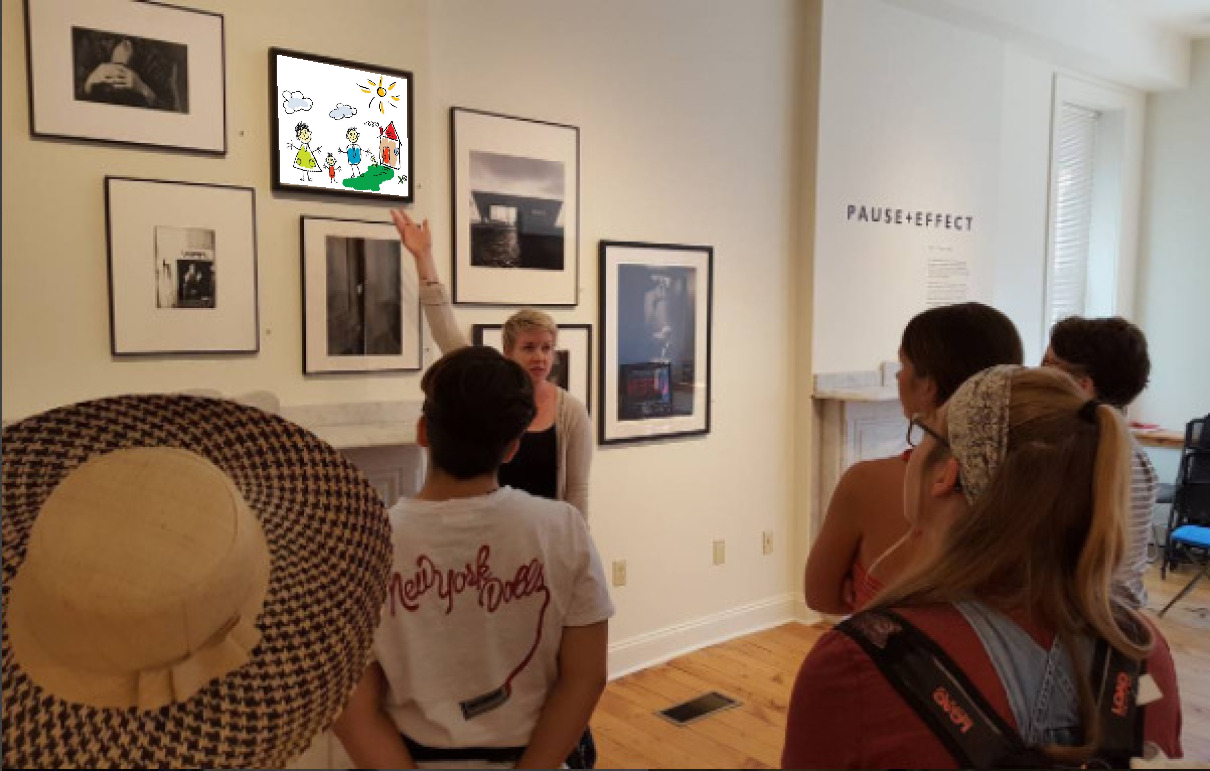
\includegraphics[height=25em]{code/outputs/prob4.png}
  \caption{Result of Problem 4}
  \label{fig:prob4}
\end{figure*}

\solution{5}
Figure \ref{fig:prob5} shows the result of problem 5.
\begin{figure*}[!h]
  \centering
  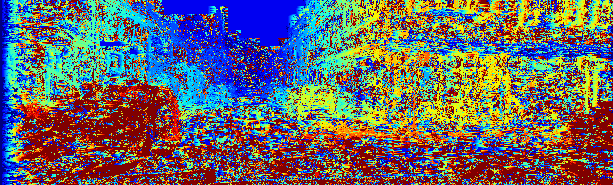
\includegraphics[height=15em]{code/outputs/prob5.png}
  \caption{Result of problem 5}
  \label{fig:prob5}
\end{figure*}


%%%%%%%%%% Important, you must edit and complete the informational
%%%%%%%%%% section below. If you discussed the problem set with no
%%%%%%%%%% one, edit it to say no discussions or external resources.
\info

This problem set took approximately 20 hours of effort.

I discussed this problem set with:
\begin{itemize}
\item Jiayao Cheng
\item Yukun Li
\end{itemize}

% Note that you might have to escape some special symbols in URLS like \_
I also got hints from the following sources:
\begin{itemize}
\item Hints from the lectures slides
\item Hints from the TA recitation and piazza
\end{itemize}

\end{document}
